\section{Introduction}\label{sec:prev}

Compression and encryption composition has caused serious security problems
in protocols such as TLS \cite{dierks2008tls} over the years
with an array of attacks making major headlines in computer security dissemination forums,
including BREACH \cite{gluck2013breach}, TIME \cite{be2013perfect}, and CRIME \cite{duong2012crime}.
While the idea that compression is a side-channel that can be exploited
is certainly folklore in the cryptography community and is documented
at least as early as Kelsey's work \cite{kelsey2002compression},
a proper theoretical model  capturing the real-world perspective
of these side-channel attacks is still elusive.

Motivated by this, in this paper we introduce
a general model that incorporates the rendering process that is exploited
during these attacks and in this way we facilitate a thorough
theoretical analysis of the security of encryption-compression composition.
We showcase the power of our approach
by (i) showing how attacks like  BREACH \cite{gluck2013breach}, TIME \cite{be2013perfect}, and CRIME \cite{duong2012crime}, can be expressed
as instances of our compression side-channel attack template,
(ii) demonstrating an improved attack framework, called Rupture,
that improves substantially the performance of previous attacks,
(iii) presenting a general mitigation strategy, called CTX, that strikes
a good balance between security and efficiency and can be readily incorporated
in a TLS deployment without a significant performance degradation.
In more details our results are outlined below.

\subsection{A high-level overview}\label{subsec:example}
As explained above,  compression side-channel attacks pose a serious threat
against real-world deployments of TLS and in general of
any encryption system. While widely received and documented
by the security community there are still not many mitigation strategies in place
to thwart them, primarily due to (i) the perceived high performance
penalty associated with mitigating them, and
(ii) their perceived complexity and
the lack of production code tools
that allow for their robust execution, something that makes some believe
they are not a realistic threat. In this work we will illustrate that
these perceptions  are wrong
and the existence of these attacks
suggests  a grave situation that is critical to be addressed.

In order to appreciate the seriousness of these attacks we present a motivating
example.
Suppose that  a  user that browses the Internet and a server
that hosts a website are in active communication.
This website might be a social network, e-banking, mail
provider or a similar service that handles sensitive private data. When the
server receives a request for a web page it collects all needed data, generates
the HTML code that will be displayed by the user's browser and sends a network
response containing this code along with other resources such as images and
libraries. All response data is encrypted under TLS, which ensures privacy and
integrity for the communication between the user and the server,
but also compressed for efficiency.

Consider now an adversary that aims to break this communication's security.
This adversary tries to decrypt the communication between
the user and the server and reveal information about the private data that is
exchanged. In order to mount a compression side-channel attack certain
conditions need to be met.

Firstly, the adversary is able to handle the user's network traffic. That way he
is able to collect and analyze the network packets of the encrypted
communication with the server. He is also able to inject code in third-party
non-encrypted HTTP responses.

Secondly, he should be able to issue any number of malicious requests using the
user's cookies (which will be encrypted). This can be achieved by forcing the user's browser to run a
piece of code, such as a Javascript script. This script can either be hosted on
an adversary-controlled website or injected in plain HTTP responses the user
receives from third websites. This script is executed when loaded in the user's
browser and is able to issue requests to any URL crafted by the adversary.
Figure \ref{fig:attack_model} elaborates further on this attack mode.

Thirdly, the web service that is under attack should allow the adversary to
inject data in the encrypted response plaintext. This data takes the form of a
specially crafted ``reflection'' string which can be added for example by using a
HTTP GET parameter whose value is included in the HTML response.

Any adversary that fulfills these requirements can issue a compression
side-channel attack against the user and the web service. The malicious requests
contain the reflection strings and the user's cookies. The response contains
both the reflection string and the user's private data. The structure of the
reflection string should depend on any known properties of the private data
to maximize the adversarial advantage.

As the attack progresses the adversary collects network data containing multiple
responses and reflections. Although this data is encrypted, analysis on the
lengths of different response packets in conjunction with the sequence
of reflections that has been used will reveal otherwise hidden properties of the private data.
At this point the privacy of the communication between the user and the website is
compromised and the adversary has broken the confidentiality of the messages
effectively circumventing TLS security.

    \begin{figure}[thpb]
        \centering
            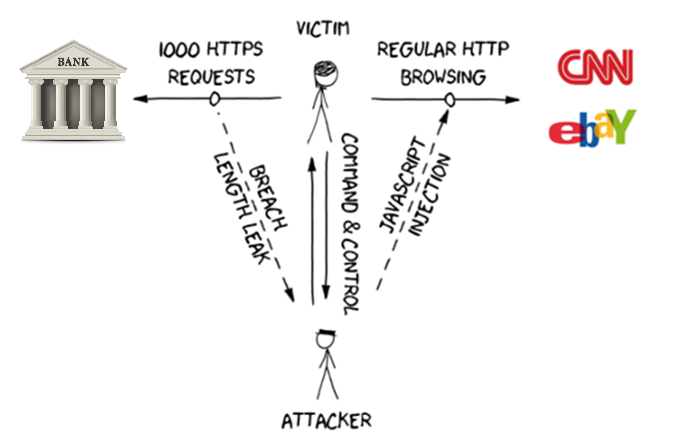
\includegraphics[width=0.48\textwidth]{figures/attack_model.png}
        \caption{The attack model}
        \label{fig:attack_model}
    \end{figure}

\subsection{A motivating example, concepts and notations}\label{subsec:terms}
We now describe a concrete example of the website in the previously described
attack to illustrate the various terms we use in the rest of this paper.  The
terms that need be explained include the \textit{rendering function} $f$,
\textit{rendered message} $m$, \textit{secret} $s$, \textit{noise} $v$,
\textit{reflection} $r$ and the distributions $\mathcal{M}$ of secrets and
$\mathcal{V}$ of noise.

In our example, the target of the attack is the website found in the URL
\textit{mail.example.com}. The victim is the user that is logged in this mail
service and whose cookies the adversary uses in his requests (and aims to learn).

The web page that the adversary exploits is
\textit{mail.example.com/search?query=attack}. This website provides a HTTP GET
parameter called \textit{query} and the adversary uses the reflection string
\textit{attack}. The HTML response is included below:

\begin{lstlisting}[basicstyle=\small\ttfamily]
<div>
    <p>You searched for: attack</p>
    <p>No results found.</p>
</div>
<div>
    Your inbox:
    <ul>
    <li>[Bank] Routing number: 123</li>
    </ul>
</div>
<div>
    <p>Current Time: 12:40:00</p>
</div>
\end{lstlisting}

The server's HTML generator is an instance of the \textit{rendering function}
$f$. This function implements the rendering of the HTML code based on
blueprints.

The output of $f$ is the \textit{rendered message} $m$. This is the generated
HTML response code that contains response data and is rendered by the user's
browser.

The HTML response contains multiple data elements. A data element can be a
\textit{secret}, \textit{noise}, \textit{static}, or a \textit{reflection}.

A \textit{secret} $s$ is any part of the response that the application wishes to
remain private. The adversary wishes to learn information about $s$. Examples of
secrets in an HTML response include private messages, email contents, financial
data, and web security elements like CSRF tokens \cite{de2011automatic}. A secret's alphabet
is generally printable text characters. In our example, the strings "Bank",
which is an email topic, and "Routing number: 123", which is the email body, are
both secrets.

A \textit{reflection} $r$ is a component crafted by the attacker and can be
adaptively transformed as the attack progresses. In our example, the HTTP GET
value "attack" of the parameter "query" is used as a reflection. This string is
included in the response in the message "You searched for: attack". This serves
as an information message for the user and reflects in every search request the
value of the GET parameter "query".

The \textit{noise} $v$ is a value that changes in every request regardless of
the requested content. Examples of noise include timestamps and ads. The noise
follows a random distribution and its alphabet consists of printable characters.
In our example, the string "12:40:00" is noise.

\textit{Static} is any content that remains unchanged across requests. Typical
examples of static data are HTML $<$div$>$ tags and CSS code. Static content is
predictable and thus irrelevant in the attack. Strings like "div", "ul", "Your
inbox:" are considered static in our example.

Secrets and reflections are chosen from the distribution $\mathcal{M}$.
$\mathcal{M}$ in our example contains all routing numbers and 4-letter strings
like "Bank".

Finally, each noise element is chosen from the distribution $\mathcal{V}$. In
our example, $\mathcal{V}$ contains all 24hr timestamps. In every request, a new
noise element is chosen from $\mathcal{V}$. In this case it is "12:40:00".

The compression function $\textrm{Com}$ is the compression algorithm used on the
HTML response plaintext. In our example, this algorithm is DEFLATE, the most
common compression algorithm in the web. The composition of $\textrm{Com}$ and
the rendering function $f$ is the encoding function $\mathcal{K}$.

The encryption function $\textrm{Enc}$ is the encryption algorithm used by the
web server during the communication. The most commonly used symmetric encryption
algorithm today is AES. We use the function $\mathcal{E}$ to describe the
composition of $\textrm{Enc}$ and $\textrm{Com}$.

The input of $\mathcal{E}$ is the message $m$ and its output is ciphertext $c$.
This ciphertext is included in the network response packets and is sniffed by
the adversary over-the-wire.

The generation of $m$, its compression and encryption and the transmission over
the network of $c$, as well as the sniffing ability of the adversary, constitute
the reflection oracle that will further described in following sections.

The adversary issues the attack in stages. In each stage he creates a pool of
reflections and makes malicious requests for each reflection in the pool. An
attack stage ends when the adversary has successfully decrypted a single
character in the secret. He then adaptively changes the reflection pool, based
on the newly stolen character, and continues similarly with the next stage.

In some cases, the adversary aims at finding a property of the secret rather
than the secret itself. This property is $g(s)$ and the guess of the adversary
is $y$. When $g(s) = y$ the adversary has successfully recognized the property
$g$ of the secret $s$. A special case of $g$ would be a predicate $Q$.

\subsection{Contributions}
Our contributions are as follows.

First we introduce a novel model for analyzing compression and encryption
composition attacks, the \textit{adaptive reflection game}, with an accompanying
security definition. This model is quite general in that it does not describe
specific instances of the rendering function $f$ or the compression function
$\textrm{Com}$. Furthermore, it allows for general distributions of secret $\mathcal{M}$
and distributions of noise $\mathcal{V}$ which can affect the rendering. Section
\ref{sec:refsec} contains the definition of this model.

We wish to prove that all encryption functions are insecure when composed with
compression. In order to produce this proof, we build a series of required
assumptions.

We define \textit{interdependence}, a property that characterizes dependent
random variables drawn from a joint distribution. Interdependence is an
important notion when exploring the effects of the reflection when compressed
with a secret. We introduce interdependence in section
\ref{subsec:interdependence}.

Another property of compression functions is \textit{compression idealness} with
respect to a message distribution. We
define idealness in theory and demonstrate how it applies on the compression
algorithms that are widely used in section \ref{subsec:com_idealness}.

Based on the properties of compression idealness and interdependence, we prove
that predicates on the secrets can be learned by choosing adversarial
reflections. We call this property \textit{compression detectability}, which we
explore in section \ref{sec:propertycom}.

The final part of our theoretical work on the attack is to show that this
somewhat innocent property directly allows the construction of an attacker,
which we prove breaks the security of the scheme in section
\ref{sec:comattack}. We also prove that such attacks can be amplified to
achieve better confidence.

At this point we implement Rupture\footnotemark[1], a production-grade open
source framework for conducting compression and encryption composition attacks.
This generic framework provides an extensible mechanism for experimentally
testing attack techniques in a modular setting. We implement specific
compression attack instances such as BREACH. This is the first time a working
tool is provided for this class of attacks.  Based on our attack framework we
achieve significant improvements in our implementation compared to previous
attempts. We improve the complexity from linear to logarithmic in the secret
alphabet's size, we attack block ciphers in addition to stream ciphers and we
employ practical techniques for network level optimization.  Rupture is further
described in section \ref{subsec:rupture}.

Having established the attack premises, we shift our interest in defending
against such attacks. Although there are several proposed defenses, we feel that
none achieves good compression performance in real-world system terms. In this
direction, we propose \textit{context hiding}, a method that mitigates a class
of practical compression side-channel attacks like BREACH. Context hiding aims
at preventing the compression detectability of a predicate $Q$ of a secret $s$
in presense of reflection as described in section \ref{sec:defense}.

Our implementation of the context hiding defense technique is called
CTX\footnote[1]{The GitHub repositories of the Rupture and CTX projects make the
source code openly available but have been removed for anonymization purposes
and can be provided upon request.}. CTX runs at the application layer of web
services and is opt-in. It is implemented in Python and Javascript and can be
used in the common web frameworks Django, Flask and Node.js. CTX achieves
balance between security and compression performance that is unprecedented
compared to other proposed defense methods.

We experimentally show in section \ref{subsubsec:ctx_experiments} that CTX
performs well in terms of size and time overhead. Specifically, we find that the
performance penalty of CTX compared to other proposed methods, like secret
masking, is significantly lower and within accepted rates for real-world
applications.
